\section{Actual rejection rates at sample size \texorpdfstring{$n$}{n}}\label{sec:finite}

\subsection{Exact finite-sample laws}
Let $x=(x_1,\dots,x_n)^\top\sim N(\mu\mathbf 1,\Gamma_n)$ with a positive definite Toeplitz covariance $\Gamma_n$, and
let $y=x-\mu_0\mathbf 1$. Each of the three statistics is a ratio $(a^\top y)^2/y^\top My$ with $a=n^{-1/2}\mathbf 1$ and a
positive semi-definite $M$ with $M\mathbf 1=0$, so that the denominator does not depend on $\mu_0$: for $T_n$,
$M=n^{-2}D^\top D$ with $D$ the matrix that maps $x$ to the demeaned partial sums $(\hat S_k)$; for $\tau_{n,m}^2$ and $t_{n,B}^2$, $M$ has rank $2m$
or $B$ and is spanned by the Fourier or cosine vectors in \eqref{eq:tauHI}--\eqref{eq:tEWC}.

\begin{proposition}[Exact finite-sample laws]\label[proposition]{prop:exactn}
Under $H_0:\mu=\mu_0$, for $c>0$, the ratio $Q=(a^\top y)^2/(y^\top My)$ satisfies $P(Q\le c)=P\big(\sum_i\theta_i(c)\xi_i^2\le0\big)$, with $\xi_i$
independent standard normal and $\theta_i(c)$ the eigenvalues of $\Gamma_n^{1/2}(aa^\top-cM)\Gamma_n^{1/2}$, of which exactly
one is positive (because $Ma=0$ and $\Gamma_n$ is positive definite). (a)~For the fixed-smoothing statistics the law depends on $\Gamma_n$ only through the $(2m+1)$- or
$(B+1)$-dimensional covariance $C^\top\Gamma_nC$ of $a^\top x$ and the coordinates. (b)~For $T_n$, if
$\Gamma_n^{1/2}M\Gamma_n^{1/2}=U\operatorname{diag}(\vartheta)U^\top$ and $\beta=U^\top\Gamma_n^{1/2}a$, the characteristic
function of $\sum_i\theta_i(c)\xi_i^2$ is
$\prod_k(1+2\mathrm isc\vartheta_k)^{-1/2}\big(1-2\mathrm is\sum_k\beta_k^2/(1+2\mathrm isc\vartheta_k)\big)^{-1/2}$, so one
eigendecomposition serves every $c$.
\end{proposition}

Part~(b) is the matrix determinant lemma; implemented via a Cholesky-free Woodbury reduction of the demeaned
cumulative-sum covariance and a two-band adaptive Imhof quadrature (\cref{sec:methods}), it requires a one-off set-up of
\pthree{e5-T3-setup-s}\,s at $n=1000$ and then \pthree{e5-T3-query-s}\,s for each further cutoff, instead of
\pthree{e5-T3-imhof-s}\,s for a fresh eigendecomposition and inversion.

\begin{proposition}[Fractional Gaussian noise]\label[proposition]{prop:fgn}
If $u_t=B_H(t)-B_H(t-1)$, then for every $n$ the vector of statistics $(T_n,\tau_{n,m},t_{n,B})$ has the law of the same
statistics computed from the increments of the fractional Brownian path $B_H$ on the grid $\{t/n\}$. In particular
$T_n\overset d=Z^2\big/\big(n^{-1}\sum_{k=1}^n\Bt(k/n)^2\big)$, the rectangle-rule discretisation of $T_H$.
\end{proposition}

Under fractional Gaussian noise the finite-sample laws are therefore pure discretisations of the limit laws, with no
short-run dynamics, and they converge rapidly: at $n=64$ and $n=128$ under fGn, the exact sizes of $T_n$ at the Brownian
cutoff $45.526$ already lie within \pthree{mx-gap-64-long}\,pp and \pthree{mx-gap-128-long}\,pp of the certified limits
for $H\in\{0.90,0.99\}$ (\pthree{mx-0.90-128}\,\% at $H=0.90$ and \pthree{mx-0.99-128}\,\% at $H=0.99$ for $n=128$),
whereas substituting the certified $H=0.99$ cutoff \pthree{mx-cv-0.99} delivers exact size \pthree{mx-0.99-64-own}\,\% at
$n=64$ and \pthree{mx-0.99-128-own}\,\% at $n=128$ (verified independently against $30$-digit Imhof integration to
\pthree{mx-maxdiff-AB}\,pp). At $n=500$ and $H=0.7$ the exact size of the Bartlett/self-normalised test at its own limit
critical value differs from $5\,\%$ by \pthree{fgn-sn-0.70-500-dev}\,pp.

\subsection{Results}
\Cref{fig:finite} and \cref{tab:finite} report exact sizes for fractional Gaussian noise, ARFIMA$(0,d,0)$ and
ARFIMA$(1,d,0)$ with $\phi=\pm0.5$, $d=H-\frac12\in\{0,\allowbreak0.1,\allowbreak0.2,\allowbreak0.3,\allowbreak0.4\}$ and $n\in\{50,\allowbreak100,\allowbreak200,\allowbreak500,\allowbreak1000,\allowbreak2000\}$,
for the Bartlett/self-normalised test, the fixed-$m$ test with $m\in\{1,2,3,4,6,8,12,16\}$ and the EWC test with
$B\in\{4,8,12,16,24,32\}$, each test using its own limit critical value at the true $H$. Three conclusions hold for all of them.

\emph{Memory alone costs little.} Under fractional Gaussian noise and ARFIMA$(0,d,0)$ every procedure is within
\pthree{fn-maxdev-pure}\,pp of $5\,\%$ for every $n\ge50$ and every $H$ in the design.

\emph{Short-run dynamics cost a lot in small samples.} With $\phi=0.5$ at $n=50$, the fixed-$m$ test with $m=16$
rejects \pthree{fn-arfima1p-HI16-0.50-50}\,\% of the time at $H=0.5$ and \pthree{fn-arfima1p-HI16-0.90-50}\,\% at
$H=0.9$, the Bartlett/self-normalised test \pthree{fn-arfima1p-SN-0.50-50}\,\% and the test with $m=1$
\pthree{fn-arfima1p-HI1-0.50-50}\,\%; with $\phi=-0.5$ the tests are conservative, down to
\pthree{fn-arfima1m-HI16-0.50-50}\,\% for $m=16$. At $n=2000$ every procedure is within \pthree{fn-maxdev-2000}\,pp.

\emph{The more components, the larger the distortion.} The ordering by the number of components is the same at every
$H$ and $n$ in the design, and the EWC test with $B=2m$ behaves like the fixed-$m$ test with $m$ frequencies.

\begin{figure}[tbp]\centering
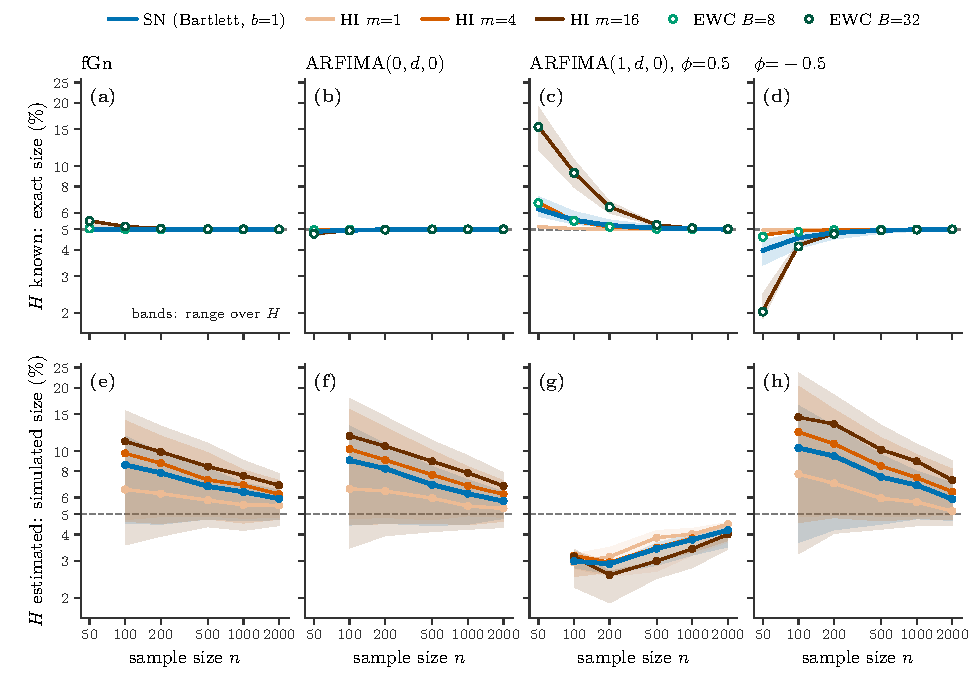
\includegraphics[width=\textwidth]{fig2_finite_n.pdf}
\caption{Finite-sample rejection rates at nominal 5\% with known memory (top) and estimated memory (bottom).}\label{fig:finite}
\end{figure}

\begin{table}[tbp]\centering\small
\caption{Exact rejection percentages at nominal 5\% using limit cutoffs at $H=0.7$.}\label{tab:finite}
\setlength{\tabcolsep}{4.5pt}\begin{tabular}{@{}llrrrrrr@{}}\toprule
model & test & $n=50$ & $n=100$ & $n=200$ & $n=500$ & $n=1000$ & $n=2000$\\\midrule
\multirow{6}{*}{fGn} & SN & 5.01 & 5.00 & 5.00 & 5.00 & 5.00 & 5.00\\
 & HI, $m=1$ & 5.00 & 5.00 & 5.00 & 5.00 & 5.00 & 5.00\\
 & HI, $m=4$ & 5.05 & 5.01 & 5.00 & 5.00 & 5.00 & 5.00\\
 & HI, $m=16$ & 5.49 & 5.16 & 5.05 & 5.01 & 5.00 & 5.00\\
 & EWC, $B=8$ & 5.05 & 5.01 & 5.00 & 5.00 & 5.00 & 5.00\\
 & EWC, $B=32$ & 5.48 & 5.16 & 5.05 & 5.01 & 5.00 & 5.00\\
\midrule
\multirow{6}{*}{ARFIMA$(0,d,0)$} & SN & 4.89 & 4.95 & 4.98 & 4.99 & 5.00 & 5.00\\
 & HI, $m=1$ & 5.00 & 5.00 & 5.00 & 5.00 & 5.00 & 5.00\\
 & HI, $m=4$ & 4.98 & 4.99 & 5.00 & 5.00 & 5.00 & 5.00\\
 & HI, $m=16$ & 4.77 & 4.94 & 4.98 & 5.00 & 5.00 & 5.00\\
 & EWC, $B=8$ & 4.97 & 4.99 & 5.00 & 5.00 & 5.00 & 5.00\\
 & EWC, $B=32$ & 4.77 & 4.94 & 4.98 & 5.00 & 5.00 & 5.00\\
\midrule
\multirow{6}{*}{ARFIMA$(1,d,0)$, $\phi=0.5$} & SN & 6.24 & 5.54 & 5.22 & 5.07 & 5.03 & 5.01\\
 & HI, $m=1$ & 5.15 & 5.04 & 5.01 & 5.00 & 5.00 & 5.00\\
 & HI, $m=4$ & 6.70 & 5.48 & 5.13 & 5.02 & 5.01 & 5.00\\
 & HI, $m=16$ & 15.44 & 9.33 & 6.40 & 5.25 & 5.07 & 5.02\\
 & EWC, $B=8$ & 6.66 & 5.49 & 5.14 & 5.03 & 5.01 & 5.00\\
 & EWC, $B=32$ & 15.38 & 9.29 & 6.39 & 5.25 & 5.07 & 5.02\\
\midrule
\multirow{6}{*}{ARFIMA$(1,d,0)$, $\phi=-0.5$} & SN & 3.97 & 4.55 & 4.82 & 4.95 & 4.98 & 4.99\\
 & HI, $m=1$ & 4.96 & 4.99 & 5.00 & 5.00 & 5.00 & 5.00\\
 & HI, $m=4$ & 4.70 & 4.91 & 4.97 & 4.99 & 5.00 & 5.00\\
 & HI, $m=16$ & 2.05 & 4.19 & 4.79 & 4.96 & 4.99 & 5.00\\
 & EWC, $B=8$ & 4.61 & 4.87 & 4.96 & 4.99 & 5.00 & 5.00\\
 & EWC, $B=32$ & 2.03 & 4.14 & 4.76 & 4.95 & 4.99 & 5.00\\

\bottomrule\end{tabular}
%
\end{table}

In \cref{fig:finite}, lines and markers follow $H=0.7$; the bands, drawn for SN and HI with $m=4$, span the grid
$H\in\{0.5,\dots,0.9\}$. Open circles mark EWC with $B=2m$. The lower panels use $40\,000$ replications per cell.

\paragraph{Validation} The exact computations were checked against independent Monte Carlo simulation with
\pthree{val-R} replications per cell, by the circulant-embedding sampler of \citet{DH87}: in
\pthree{val-n-inside} of \pthree{val-n-cells} cells the exact rate lies inside the $99\,\%$ Wilson interval, and the
standardised differences have mean \pthree{val-z-mean} and standard deviation \pthree{val-z-sd}, as they should if the
exact rates are correct (Supplementary Material Figure~S.1). A second, larger check comes from the estimated-$H$ study
below, whose \emph{oracle} rule uses the critical value at the true $H$: over its \pthree{or-n-cells} cells (four
models, $n=100,\dots,2000$, three levels) the exact rate lies inside the $99\,\%$ interval in \pthree{or-inside-pct}\,\%
of them, with standardised differences of mean \pthree{or-z-mean}, standard deviation \pthree{or-z-sd} and largest
absolute value \pthree{or-maxz}. The exact laws also reproduce the published rejection frequencies of
\citet[Table~2]{HI17} for the AR(1) design with $\phi=0.5$ at $T=64$ and $256$, with largest standardised difference
\pthree{hi17-t2-maxz} over the \pthree{hi17-t2-n} published cells.

\subsection{When \texorpdfstring{$H$}{H} is estimated}\label{sec:plugin}
In practice $H$ is unknown. We first estimate it by the local Whittle estimator \citep{Rob95} with bandwidth
$m_{\mathrm{LW}}=\lfloor n^{0.65}\rfloor$, as in \citet{HI17}, and plug the estimate into the limit critical value;
these rates are simulated. Reproducing Tables~3--5 of \citet{HI17}---Gaussian ARFIMA$(1,\delta,0)$ with
$(\delta,\phi)\in\{(0,0),(-0.3,0.5),(0.3,-0.5)\}$ and \pthree{hi17-R} replications (Supplementary Material Table~S.3)---confirms
their plug-in pattern: linearly interpolating their printed Table~1 differs from their published rates by
\pthree{hi17-meandiff}\,pp on average (\pthree{hi17-share-z2}\,\% of the \pthree{hi17-ncells} cells beyond two joint
standard errors, maximum \pthree{hi17-maxdiff}\,pp). The published description does not identify the source of the residual differences. Pairing those
plug-in rates with the \emph{exact} finite-$T$ oracle sizes from \cref{prop:exactn} (Supplementary Material Table~S.3)
yields the central decomposition: with the true $\delta$ the fixed-$m$ test stays close to nominal (exactly $5.00\,\%$
under white noise), whereas with estimated $\delta$ the size reaches \pthree{hi17-T5-64-16-plugin}\,\% at $T=64$ in
their Table~5. On this grid the contrast measures the effect of estimating $H$ while holding the design and statistic fixed.

The same decomposition holds across our full design grid (\cref{fig:finite}, bottom row, and \cref{tab:plugin}), with
\pthree{pl-R} replications per cell and $\hat H$ clipped to $[\frac12,0.99]$ for every test so that all procedures
assume long memory a priori in the same way. Under fractional Gaussian noise and ARFIMA$(0,d,0)$ with $H\ge0.6$ the
feasible tests reject between \pthree{pl-pure-min-100} and \pthree{pl-pure-max-100}\,\% at $n=100$ and between
\pthree{pl-pure-min-2000} and \pthree{pl-pure-max-2000}\,\% at $n=2000$ (over $H\in\{0.6,0.7,0.8,0.9\}$), against at
most \pthree{fn-maxdev-pure}\,pp of distortion when $H$ is known. At $H=0.9$ and $n=100$ under fractional Gaussian noise
the Bartlett/self-normalised test rejects \pthree{pl-fgn-SN-0.9-100}\,\%, the fixed-$m$ test with $m=4$
\pthree{pl-fgn-HI4-0.9-100}\,\% and with $m=16$ \pthree{pl-fgn-HI16-0.9-100}\,\%. With estimated $H$ the distortion
grows with the number of components: in the \pthree{pl-n-pure-cells} pure-memory cells with $H\ge0.6$, HI with $m=1$
is less distorted than SN in \pthree{pl-share-hi1-le-sn}\,\% of cells and EWC with $B=4$ in \pthree{pl-share-ewc4-le-sn}\,\%,
whereas SN is less distorted than HI with $m=4$ and $16$ in \pthree{pl-share-sn-le-hi4}\,\% and than EWC with $B=8$ and $32$
in \pthree{pl-share-sn-le-ewc8}\,\%. The power ranking of \cref{sec:power} therefore comes with the opposite ranking in
feasible size. Positive short-run correlation biases $\hat H$ upwards and makes every feasible test conservative (sizes
between \pthree{pl-ar1p-min} and \pthree{pl-ar1p-max}\,\%); negative correlation biases $\hat H$ downwards, pushing
rejection rates up to \pthree{pl-ar1m-max-100}\,\% at $n=100$. Clipping matters only near $H=\frac12$: at $H=0.5$,
$n=100$, HI with $m=4$ rejects \pthree{pl-HI4-H05-trunc}\,\% with clipped $\hat H$ versus \pthree{pl-HI4-H05-untrunc}\,\%
unclipped.

\paragraph{Bandwidth sensitivity} Across local Whittle bandwidths $\lfloor n^{0.5}\rfloor$, $\lfloor n^{0.65}\rfloor$
and $\lfloor n^{0.8}\rfloor$ (common random numbers; full table in Supplementary Material Table~S.4), feasible sizes
under pure long memory ($H\in\{0.7,0.9\}$) span \pthree{bw-50-min-100}--\pthree{bw-50-max-100}\,\%,
\pthree{bw-65-min-100}--\pthree{bw-65-max-100}\,\% and \pthree{bw-80-min-100}--\pthree{bw-80-max-100}\,\% at $n=100$,
and \pthree{bw-50-min-2000}--\pthree{bw-50-max-2000}\,\%, \pthree{bw-65-min-2000}--\pthree{bw-65-max-2000}\,\% and
\pthree{bw-80-min-2000}--\pthree{bw-80-max-2000}\,\% at $n=2000$. Widening the bandwidth to $n^{0.8}$ lowers estimator
variance enough to keep fGn within \pthree{bw-80-fgn-maxdev-500}\,pp of nominal from $n=500$, but leaves ARFIMA$(0,d,0)$
distorted up to \pthree{bw-80-arfima0-max-500}\,\% and amplifies short-run bias \citep{Rob95}.

\begin{table}[tbp]\centering\small
\caption{Simulated rejection percentages at nominal 5\% using local Whittle estimates of memory.}\label{tab:plugin}
\begin{tabular}{@{}llrrrrrr@{}}\toprule
& & \multicolumn{3}{c}{$H=0.7$} & \multicolumn{3}{c}{$H=0.9$}\\\cmidrule(lr){3-5}\cmidrule(l){6-8}
model & test & $n=100$ & $500$ & $2000$ & $n=100$ & $500$ & $2000$\\\midrule
fGn & SN & 8.6 & 6.8 & 5.9 & 11.8 & 8.3 & 6.5\\
 & HI, $m=4$ & 9.7 & 7.3 & 6.2 & 14.0 & 9.8 & 7.2\\
 & HI, $m=16$ & 11.1 & 8.4 & 6.9 & 15.6 & 10.9 & 7.8\\
 & EWC, $B=8$ & 9.6 & 7.3 & 6.2 & 13.8 & 9.8 & 7.3\\
 & EWC, $B=32$ & 11.1 & 8.4 & 6.8 & 15.6 & 10.9 & 7.8\\
\addlinespace
ARFIMA$(0,d,0)$ & SN & 9.0 & 6.9 & 5.8 & 13.2 & 8.4 & 6.4\\
 & HI, $m=4$ & 10.2 & 7.7 & 6.2 & 15.8 & 10.1 & 7.2\\
 & HI, $m=16$ & 11.8 & 8.9 & 6.8 & 17.8 & 11.2 & 7.9\\
 & EWC, $B=8$ & 10.1 & 7.7 & 6.2 & 15.6 & 10.0 & 7.2\\
 & EWC, $B=32$ & 11.8 & 9.0 & 6.8 & 17.8 & 11.2 & 7.9\\
\addlinespace
ARFIMA$(1,d,0)$, $\phi=0.5$ & SN & 3.0 & 3.4 & 4.2 & 3.1 & 2.9 & 3.5\\
 & HI, $m=4$ & 3.2 & 3.5 & 4.1 & 3.4 & 3.0 & 3.7\\
 & HI, $m=16$ & 3.1 & 3.0 & 4.0 & 3.4 & 2.9 & 3.7\\
 & EWC, $B=8$ & 3.1 & 3.4 & 4.2 & 3.2 & 3.0 & 3.8\\
 & EWC, $B=32$ & 3.1 & 3.0 & 4.0 & 3.4 & 2.9 & 3.7\\
\addlinespace
ARFIMA$(1,d,0)$, $\phi=-0.5$ & SN & 10.3 & 7.5 & 5.9 & 16.4 & 9.6 & 7.0\\
 & HI, $m=4$ & 12.3 & 8.5 & 6.4 & 20.4 & 11.6 & 8.2\\
 & HI, $m=16$ & 14.5 & 10.1 & 7.3 & 23.5 & 13.3 & 9.0\\
 & EWC, $B=8$ & 12.2 & 8.4 & 6.5 & 20.2 & 11.5 & 8.1\\
 & EWC, $B=32$ & 14.3 & 10.1 & 7.3 & 23.5 & 13.3 & 9.0\\
\bottomrule\end{tabular}
%
\end{table}

\subsection{Competitor baselines and practical remedies under unknown \texorpdfstring{$H$}{H}}\label{sec:competitors}
We compare \CosCert{} plug-in rules, all with $\hat H$ truncated to $[\frac12,0.99]$ as in \cref{sec:plugin}, with four
feasible alternatives in \cref{tab:competitors} ($20\,000$ replications per design,
$n\in\{100,500\}$, $H\in\{0.5,0.7,0.9\}$, all four data models, measuring both null size and finite-sample local power
at $\mu_n=2.8\sqrt{\Var(\bar x_n)}$, where the Gaussian known-variance $z$-test has approximately $80\,\%$ power in every
design):
(i)~\emph{Exact Local Whittle (ELW) plug-in}---replacing Robinson's local Whittle with the demeaned exact local Whittle
estimator $\hat H_{\mathrm{ELW}}$ of \citet{SP05} and \citet{Shi10};
(ii)~\emph{Upper-confidence-bound plug-in}---evaluating \CosCert{} at the one-sided $90\,\%$ upper confidence bound
$\hat H_{\mathrm{up}}=\min\big(0.99,\,\hat H_{\mathrm{LW}}+z_{0.90}/(2\sqrt{m_{\mathrm{LW}}})\big)$ to guard directly
against downward estimation errors in $\hat H$;
(iii)~\emph{Memory- and autocorrelation-consistent (ADG--MAC) Studentisation} \citep{ADG09}---forming
$t_{\mathrm{MAC}}=n^{1/2-\hat d}\bar x/\hat V_{\mathrm{MAC}}^{1/2}$ with
$\hat V_{\mathrm{MAC}}=(2\pi\hat G)\,\Gamma(1-2\hat d)/\{(2\hat d+1)\Gamma(1+\hat d)\Gamma(1-\hat d)\}$ and
comparing $|t_{\mathrm{MAC}}|$ against $z_{0.975}=1.96$; and
(iv)~\emph{Rate-free self-normalised subsampling} \citep{PRW99,Sha10}---comparing $T_n$ against the empirical
distribution of overlapping centred sub-blocks $T_b^{(i)}$ of length $b=\operatorname{round}(n^{0.6})$ without
estimating $H$ at all.

\begin{table}[tbp]\centering\small
\caption{Simulated size and local power of feasible tests, in percent, at nominal 5\%.}\label{tab:competitors}
\footnotesize\setlength{\tabcolsep}{2.6pt}\begin{tabular}{@{}lcccccc@{}}\toprule
 & \multicolumn{2}{c}{fGn ($H=0.7$)} & \multicolumn{2}{c}{fGn ($H=0.9$)} & \multicolumn{1}{c}{$\phi{=}0.5$, $H{=}0.7$} & \multicolumn{1}{c}{$\phi{=}-0.5$, $H{=}0.7$}\\
\cmidrule(lr){2-3}\cmidrule(lr){4-5}\cmidrule(lr){6-6}\cmidrule(l){7-7}
procedure (size / power) & $n=100$ & $500$ & $n=100$ & $500$ & $n=500$ & $n=500$\\\midrule
SN (\CosCert{} LW) & 8.6 / 50.3 & 6.8 / 52.2 & 11.7 / 43.1 & 8.0 / 44.1 & 3.3 / 35.8 & 7.4 / 55.4\\
SN (\CosCert{} Upper-CI) & 4.5 / 31.2 & 3.8 / 37.9 & 4.9 / 20.1 & 3.3 / 21.7 & 1.5 / 20.8 & 4.4 / 41.6\\
HI $m{=}4$ (\CosCert{} LW) & 9.7 / 58.3 & 7.5 / 62.9 & 14.0 / 49.5 & 9.5 / 53.2 & 3.3 / 41.4 & 8.5 / 66.3\\
HI $m{=}4$ (\CosCert{} ELW) & 8.5 / 53.9 & 7.1 / 61.7 & 11.6 / 43.5 & 8.9 / 51.7 & 3.0 / 39.8 & 8.1 / 65.5\\
HI $m{=}4$ (\CosCert{} Upper-CI) & 4.6 / 34.5 & 3.8 / 44.2 & 5.5 / 22.0 & 3.6 / 25.1 & 1.2 / 22.4 & 4.5 / 48.7\\
EWC $B{=}8$ (\CosCert{} LW) & 9.6 / 58.3 & 7.5 / 62.6 & 13.9 / 49.5 & 9.4 / 53.2 & 3.3 / 41.5 & 8.5 / 66.3\\
ADG--MAC ($N(0,1)$) & 13.5 / 64.9 & 9.4 / 70.3 & 16.4 / 53.0 & 11.2 / 58.5 & 3.0 / 42.3 & 11.0 / 75.3\\
Subsampling SN (rate-free) & 15.8 / 67.6 & 11.3 / 62.4 & 27.8 / 79.0 & 20.5 / 72.9 & 9.5 / 57.2 & 12.6 / 66.1\\
\bottomrule\end{tabular}
%
\end{table}

\Cref{tab:competitors} reports six of the \pthree{comp-n-designs} designs. For the fixed-$m$ test with $m=4$, replacing
local Whittle (LW) by demeaned exact local Whittle (ELW) moves the simulated size closer to $5\,\%$ in exactly the
\pthree{comp-elw-closer} designs with $H>\frac12$ and no positive short-run correlation. In the other
\pthree{comp-elw-further} designs the LW rule already rejects too rarely---under positive AR, and at $H=\frac12$, where
truncation holds it at \pthree{comp-hi4-lw-h05-min}--\pthree{comp-hi4-lw-h05-max}\,\%---and ELW lowers rejection further.
Under fractional Gaussian noise at $H=0.9$ and $n=100$, ELW reduces size from \pthree{comp-hi4-lw-fgn-09-100}\,\% to
\pthree{comp-hi4-elw-fgn-09-100}\,\%.

For the four-frequency test, the upper-confidence-bound rule reduces rejection. At $n=500$ its simulated size is at most
\pthree{comp-hi4-up-n500-max}\,\% in all \pthree{comp-n500-designs} designs, against up to \pthree{comp-hi4-lw-n500-max}\,\%
for the LW rule and \pthree{comp-hi4-elw-n500-max}\,\% for the ELW rule. At $n=100$ it cuts the worst case, the
negative-AR design at $H=0.9$, from \pthree{comp-hi4-lw-ar1m-09-100}\,\% to \pthree{comp-hi4-up-ar1m-09-100}\,\%. The price
is power: under fractional Gaussian noise at $H=0.7$ and $n=500$, power falls from \pthree{comp-hi4-lw-fgn-07-500-pw}\,\%
to \pthree{comp-hi4-up-fgn-07-500-pw}\,\%.

At $H=0.9$ under fractional Gaussian noise, subsampling rejected a true null in \pthree{comp-sub-fgn-09-100}\,\% of
samples at $n=100$ and \pthree{comp-sub-fgn-09-500}\,\% at $n=500$. MAC and subsampling also had higher rejection
under the alternative in several designs. These are raw powers at a common nominal level, so differences in actual
size contribute to the comparison.
